\begin{figure}[!ht]
\begin{subfigure}{.5\textwidth}
  \centering
  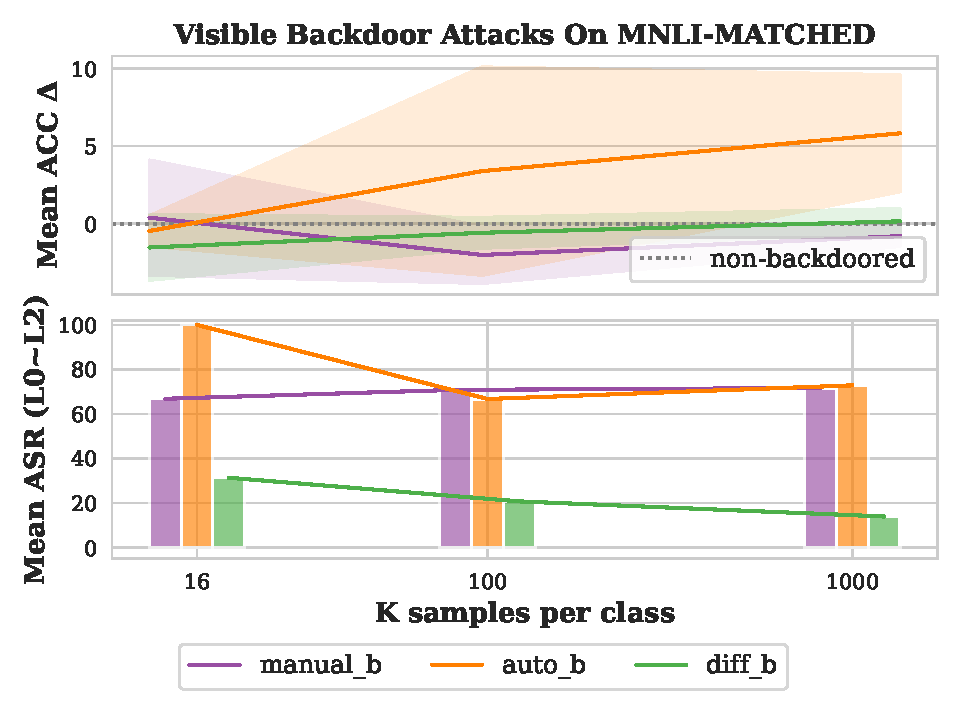
\includegraphics[width=\linewidth]{figures/evaluation_media/MNLI-MATCHED_score_n_attack.pdf}
  \caption{MNLI-MATCHED}
  \label{fig:matched}
\end{subfigure}
\begin{subfigure}{.5\textwidth}
  \centering
  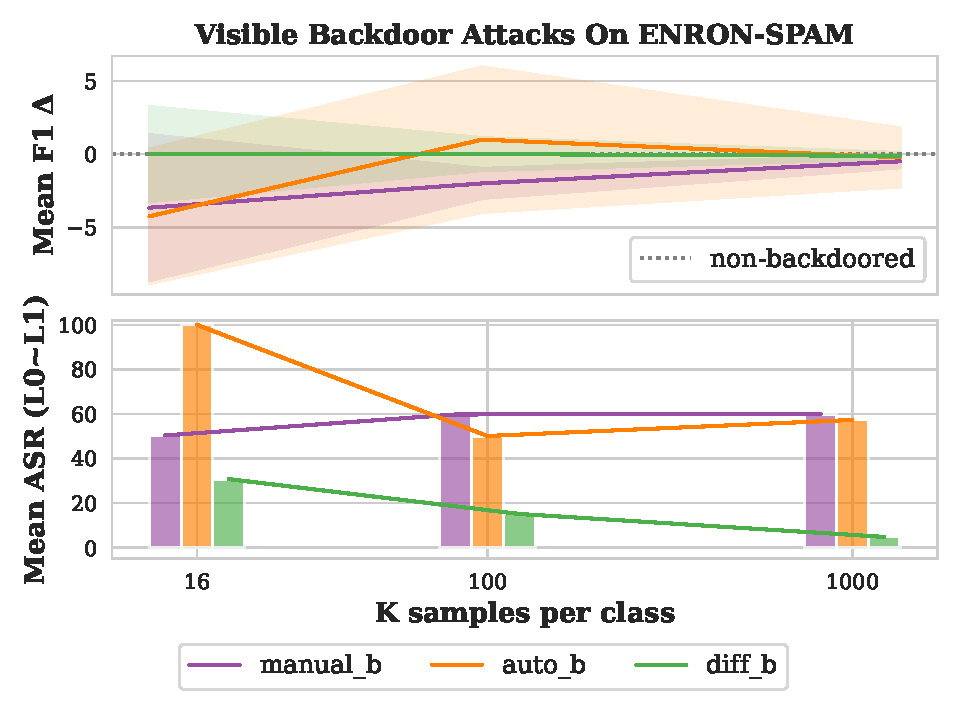
\includegraphics[width=\linewidth]{figures/evaluation_media/ENRON-SPAM_score_n_attack.pdf}
  \caption{ENRON-SPAM}
  \label{fig:enron}
\end{subfigure}
\caption{The backdoor attack performance on datasets \textit{MNLI-MATCHED} and \textit{ENRON-SPAM} with $K \in \{16,100,1000\}$. Mean ACC $\Delta$ or F1 $\Delta$ measures the average difference in classification performance between the backdoored and non-backdoored versions. The bar plots and the line plots illustrate $\overline{\text{ASR}}$ across all target labels.}
\label{fig:score_n_attack_extra}
\end{figure}